\chapter{Arquitetura física}

\section{Uso de memória}

A Tabela \ref{tab:uso_memoria} apresenta o uso estimado das memórias RAM e flash do Kit LPC1768 para o desenvolvimento do sistema. Considerou-se na estimativa apenas os componentes que já estavam disponíveis ao projeto anteriormente (CMSIS RTOS e driver da UART). Pela análise, como a maior parte das memórias permanece livre, considera-se que a quantidade é suficiente para o desenvolvimento dos componentes restantes do sistema.

\begin{table}[h!]
	\caption{Uso estimado das memórias do Kit LPC1768.}
	\centering
	\begin{tabular}{|c|c|c|}
		\hline
		\textbf{} &\textbf{RAM (64 kB máx.)} & \textbf{Flash (512 kB máx.)} \\ \hline \hline
		CMSIS RTOS & 2600 B & 5400 B\\
		Driver da UART & 150 B & 800 B\\
		\hline
		\bf{Total ocupado} & 2750 B (2.68 kB) & 6200 B (6.05 kB)\\
		\bf{Total Livre} & 61.32 kB (95.81\%) & 505.95 kB (98.82\%) \\
		\hline
	\end{tabular}
	\label{tab:uso_memoria}
\end{table}


\section{Diagrama de objetos}



\section{Projeto dos componentes}

A Figura \ref{fig:maq_estados} apresenta um diagrama de estados, contendo a visão geral do funcionamento do sistema. O estado ``Inicialização'' compreende todas as funções que são necessárias para iniciar a operação do sistema (como por exemplo, inicializar o driver da UART, sistema operacional, variáveis internas, entre outros). O estado ``Ocioso'' representa a situação em que o elevador não possui requisições pendentes, sendo que neste caso ele permanece parado no mesmo andar e com as portas abertas. 

Os estados ``Subindo'' e ``Descendo'' são muito similares internamente, ambos representado situações em que o elevador está atendendo a requisições de usuários. A diferença está essencialmente na direção de movimento do elevador. Os seus sub-estados especificam o modo de operação do elevador para atender às demandas de deslocamento até os andares requisitados. Todas as requisições de usuários são enfileiradas por prioridade, em uma tarefa separada (enfileirador). O próximo andar que o elevador deve ir fica sempre no topo da fila, sendo que as a maioria das decisões e transições nos estados e sub-estados depende de qual é este andar.

A comunicação com o computador (executanto a simulação de elevador) está presente de forma implícita no diagrama, o que inclui o recebimento de requisições de botões, recebimento de informações de posição do elevador e envio de comandos ao elevador e portas.

\begin{figure}[h]
    \centering
    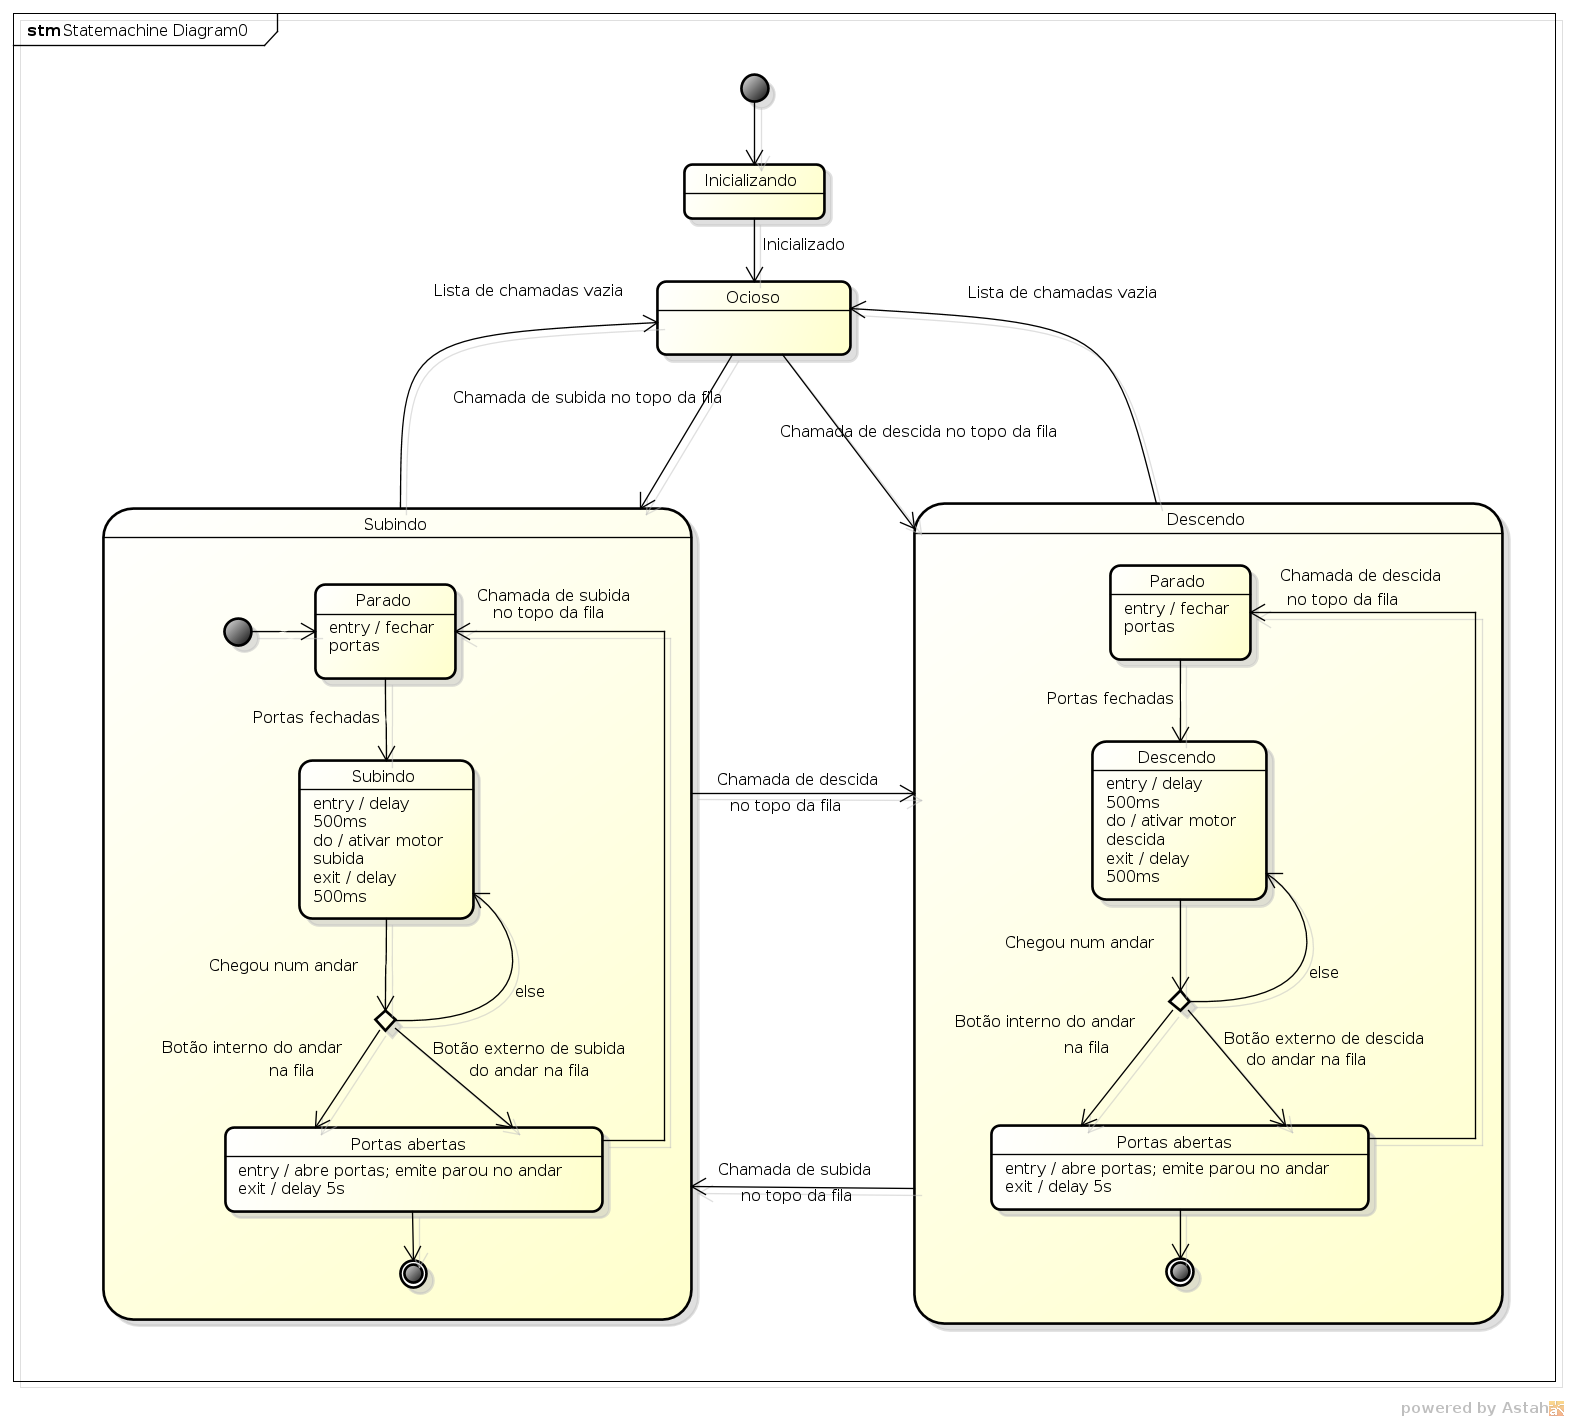
\includegraphics[width=1\columnwidth]{./figures/maq_estados.png}
    \caption{Diagrama de estados geral do sistema.}
    \label{fig:maq_estados}
\end{figure}




